\documentclass[tikz,border=2pt]{standalone}
\usepackage{ctex}
\usetikzlibrary{calc}
\begin{document}
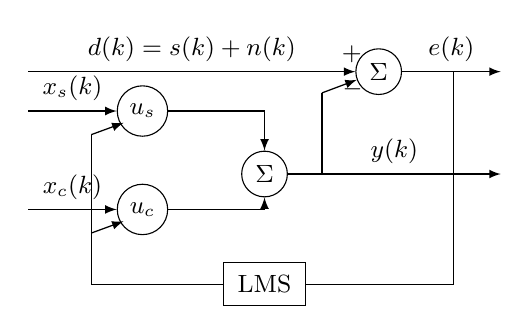
\begin{tikzpicture}[
  >=latex,
  font=\small,
  line/.style={draw, -latex, line width=0.45pt},
  plain/.style={draw, line width=0.45pt},
  sum/.style={draw, circle, minimum size=0.58cm, inner sep=0pt},
  gain/.style={draw, circle, minimum size=0.64cm, inner sep=0pt},
  block/.style={draw, rectangle, minimum width=1.05cm, minimum height=0.55cm, align=center}
]
\node[gain] (us) at (2.0,2.35) {$u_s$};
\node[gain] (uc) at (2.0,1.10) {$u_c$};
\node[sum] (sumy) at (3.55,1.55) {$\Sigma$};
\node[sum] (sume) at (5.0,2.85) {$\Sigma$};
\node[block] (lms) at (3.55,0.15) {LMS};

\draw[line] (0.55,2.35) -- node[above] {$x_s(k)$} (us);
\draw[line] (0.55,1.10) -- node[above] {$x_c(k)$} (uc);
\draw[line] (us) -| (sumy);
\draw[line] (uc) -| (sumy);
\draw[line] (0.55,2.85) -- node[above] {$d(k)=s(k)+n(k)$} (sume);
\draw[line] (sumy) -- node[above] {$y(k)$} (6.55,1.55);
\draw[plain] (4.28,1.55) -- (4.28,2.58);
\draw[line] (4.28,2.58) -- (sume);
\node at (4.67,2.62) {$-$};
\node at (4.66,3.07) {$+$};
\draw[line] (sume) -- node[above] {$e(k)$} (6.55,2.85);

\draw[plain] (5.95,2.85) -- (5.95,0.15) -- (4.08,0.15);
\draw[plain] (3.02,0.15) -- (1.35,0.15) -- (1.35,2.05);
\draw[plain] (1.35,0.15) -- (1.35,0.80);
\draw[line] (1.35,2.05) -- (1.76,2.20);
\draw[line] (1.35,0.80) -- (1.76,0.95);
\end{tikzpicture}
\end{document}
